\pagebreak
\section{Mikrocontroller}
    Die zentrale Steuereinheit der Wetterstation wird durch einen \emph{STM8L152} Mikrocontroller von ST Microelectronics gebildet. Dieser ist zusammen mit einer 3.3V Spannungsversorgung, einem Quarzoszillator und einem Debug- und Programmieradapter auf einer kommerziell erhältlichen Entwicklungsplatine montiert. Die Verbindung zu den anwendungsspezifischen Modulen der Wetterstation geschieht über zwei zweireihige 38-pin Stiftleisten.
    
    Die Anschlussbelegung der \emph{Nucleo-64} Entwicklungsplatine ist standardisiert \cite{st_nucleo}; neben dem hier verwendeten \emph{STM8} Mikrocontroller bietet ST Microelectronics Entwicklungsplatinen in diesem Formfaktor für eine Reihe von Controllerfamilien an.
    
    \subsection{Auswahl des Mikrocontrollersystems}
    In der Voruntersuchungsphase des Projektes wurden unterschiedliche Mikrocontrollersysteme für den Einsatz in der Wetterstation untersucht. Hierbei konnte auf bereits vorliegende Hardware zugegriffen werden. Folgende Controllerfamilien wurden ausgewertet:
    \begin{itemize}
        \item Atmel, 8-bit AVR: ATmega328P (Arduino Uno)
        \item Atmel, 8-bit AVR: ATmega2560 (Arduino Mega)
        \item Atmel, 32-bit ARM Cortex-M3: SAM3X8E (Arduino Due)
        \item ST Microelectronics, 32-bit ARM Cortex-M4F: STM32F446 (NUCLEO-F446RE)
        \item ST Microelectronics, 8-bit STM8: STM8L152R8 (NUCLEO-8L152R8)
    \end{itemize}
    
    Für die Auswahl wurde neben den Hardwarespezifikationen auch die Qualität der Software-Werkzeuge und der Entwicklungskomfort in Betracht gezogen. Die Ergebnisse sind nachfolgend in der Entscheidungsmatrix (s. Tab.~\ref{tab:mcu_auswahl_hardware} und~\ref{tab:mcu_auswahl_ide}) aufgezeichnet.
    
    \begin{table}[H]
        \centering
        \begin{tabular}{|l|c|c|c|c|c|}
            \hline
            \textbf{Controller} & \textbf{UART} & \textbf{SPI} & \textbf{I\textsuperscript{2}C} & \textbf{Analog In} & \textbf{Sleep I\textsubscript{CC}}\\
            \hline
            ATmega328P~\cite{ds_atmega328p} & 1 & 1 & 1 & 6  & 4 mA  \\
            ATmega2560~\cite{ds_atmega2560} & 4 & 1 & 1 & 16 & 7 mA  \\
            SAM3X8E~\cite{ds_sam3x8e}       & 5 & 4 & 2 & 16 & 8 mA  \\
            STM32F446RE~\cite{ds_stm32f446} & 6 & 4 & 4 & 16 & 10 mA \\
            STM8L152R8~\cite{ds_stm8l152r8} & 3 & 2 & 1 & 28 & 4 mA  \\
            \hline
        \end{tabular}
        \caption{Entscheidungsmatrix für die Auswahl des Mikrocontrollersystems (Hardwarespezifikationen)}
        \label{tab:mcu_auswahl_hardware}
    \end{table}
    \begin{table}[H]
        \centering
        \begin{tabular}{|l|c|c|c|c|c|c|}
            \hline
            \textbf{Controller} & \textbf{IDE} & \textbf{Debugger}  & \textbf{MCU} & \textbf{Perhiph.} & \textbf{Sleep} & \textbf{Aufwand} \\
            \textbf{} & \textbf{} & \textbf{} & \textbf{Library} & \textbf{Library} & \textbf{} & \textbf{} \\
            \hline
            ATmega328P          & Arduino IDE  & nein & Arduino & ja & nein & sehr einfach \\
            ATmega328P          & Atmel Studio & ja (ext) & ASF & nein & ja & einfach \\
            ATmega2560          & Arduino IDE  & nein & Arduino & ja & nein & sehr einfach \\
            ATmega2560          & Atmel Studio & ja (ext) & ASF & nein & ja & hoch \\
            SAM3X8E             & Atmel Studio & ja (ext) & ASF & nein & ja & sehr hoch \\
            STM32F446RE         & TrueStudio & ja & CMSIS & nein & ja & sehr hoch \\
            STM8L152R8          & STVD & ja & STM8-SPL & nein & ja & einfach \\
            \hline
        \end{tabular}
        \caption{Entscheidungsmatrix für die Auswahl des Mikrocontrollersystems (Entwicklungsumgebung)}
        \label{tab:mcu_auswahl_ide}
    \end{table}

    Ausgehend hiervon wurde die Entscheidung getroffen, den \emph{STM8L152R8} Mikrocontroller für das Projekt einzusetzen. Der primäre Kandidat, \emph{ATmega328P} konnte aufgrund der zu geringen Anzahl von UART-Schnittstellen nicht eingesetzt werden.
    
    \subsection{Pin-Belegung}
    Für die Planung der Pin-Belegung wurde das Tool \emph{STM8CubeMX} eingesetzt (s. Abb.~\ref{fig:mcu_pins}), welches neben der Pin-Zuordnung auch die Konfiguration des Clock Tree dokumentieren kann und ein Analysewerkzeug für die Leistungsaufnahme bereitstellt.
    
    Aus der grafischen Visualisierung des Controller-IC ist zu erkennen, dass die Anzahl der verfügbaren I/Os gerade optimal für diesen Anwendungsfall ist -- der Controller ist also weder überdimensioniert, noch mussten Abstriche an den I/Os gemacht werden.
    
    \begin{figure}[H]
        \centering
        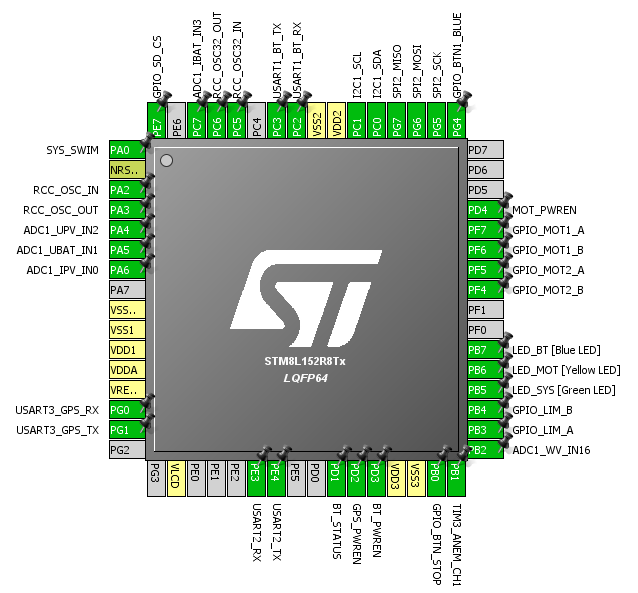
\includegraphics[width=.8\textwidth]{./img/stm8_pinout.PNG}
        \caption{Pin-Zuordnungen für den STM8-Mikrocontroller}
        \label{fig:mcu_pins}
    \end{figure}

    \begin{table}[H]
        \centering
        \begin{tabular}{|l|l|}
            \hline
            \textbf{Peripheral} & \textbf{Verwendung}                   \\
            \hline
            ADC1                & CPU-Temperatursensor,  Strom- und     \\
                                & Spannungssensoren, Richtungssignal    \\
                                & Windfahne                             \\
            GPIO                & Taster, LEDs, Endlagenschalter, Motor-\\
                                & treiber Steuersignale                 \\
            I2C                 & Digitale Sensoren                     \\
            SPI2                & SD-Karte                              \\
            TIM3                & Zähler für Anemometer-Geberimpulse    \\
            UART1               & UART-over-Bluetooth Umsetzer          \\
            UART2               & printf()-Debugausgaben                \\
            UART3               & NMEA 0183 Sentences vom GPS-Modul     \\
            \hline
        \end{tabular}
        \caption{Mikrocontroller-Peripheriemodule und ihr Einsatzzweck für die Wetterstation}
    \end{table}    

\pagebreak
\section{Firmware}\label{cha:C-Code}
    Die entwickelte Mikrocontroller-Firmware definiert den Funktionsumfang der Wetterstation: neben der Auswertung und Aufzeichnung von Messdaten erfolgt die Ausrichtung des Solarpanels softwaregesteuert.
    
    Das Softwareprojekt ist dabei modular aufgebaut -- voneinander unabhängige Softwarekomponenten sind in eigene Module aufgeteilt. Funktionen zur Umrechnung der rohen Sensordaten in die gewünschten Darstellungen werden durch entsprechende Unterteilung in verschiedene Headerdateien vor anderen Teilen der Software ``versteckt''.
    
    Hieraus wurde eine die folgende Projektstruktur entwickelt:
    \begin{itemize}
        \item \texttt{main} -- Initialisierung des Systems beim Start und zyklische Datenverarbeitung im Hintergrund-Task
        \item \texttt{commlib/} -- Module zur Ansteuerung der seriellen Kommunikationsschnittstellen (UART, SPI, I\textsuperscript{2}C)
        \item \texttt{fslib/} -- Implementierung des FAT-Dateisystems für die SD-Karte, basierend auf der Open-Source Bibliothek ``FatFS''~\cite{elmchan_fatfs}
        \item \texttt{motorlib/} -- Motorsteuerung mit Reaktion auf Betätigung der Endlagenschalter in einer Interruptserviceroutine
        \item \texttt{powerlib/} -- C-Präprozessormakros für den Wechsel in den ``wait-for-interrupt'' Wartezustand
        \item \texttt{sensorlib/} -- Module zur Auswertung der digitalen und analogen Sensoren
        \item \texttt{stm8lib/} -- STM8 Standard Peripheral Library vom Mikrocontroller-Hersteller ST Microelectronics
        \item \texttt{userlib/} -- Module zur Steuerung des Systems auf einer höheren Abstraktionsebene
    \end{itemize}

    Die Software wurde dabei für eine interruptgesteuerte Verarbeitung ausgelegt. Der Mikrocontroller wird durch Timer-Interrupts in regelmäßigen Zeitabständen ``aufgeweckt'', um Steuerungsaufgaben auszuführen. Nach Abschluss der Ausführung wird er wieder in den Wartezustand ``wait-for-interrupt'' versetzt, um die Stromaufnahme während der Leerlaufzeit zu verringern.
    
    \subsection{Auswertung der Sensoren (\texttt{sensorlib})}
    In diesem Abschnitt wird die firmwareseitige Konfiguration und Auswertung einiger der verwendeten Sensoren beschrieben.
    
        \subsubsection{BME280}\label{ssec:BME280}
            Der BME280 Klimasensor kommuniziert über eine I\textsuperscript{2}C-Schnittstelle mit dem Mikrocontroller. In der Initialisierungsphase des Systems wird der Sensor zunächst über einen \emph{Reset}-Befehl auf seinen Einschaltzustand zurückgesetzt. Anschließend werden die im nichtflüchtigen Speicher des Sensors programmierten Kalibrierungswerte für die Temperatur-, Luftfeuchte- und Luftdruckmung ausgelesen. Der Sensor wird bereits im kalibrierten Zustand durch den Hersteller ausgeliefert.
            
            \paragraph{Sleep-Mode und Messwerterfassung}\mbox{}\\
            Nach dem Reset befindet sich der Sensor im ``Sleep''-Mode, und es findet keine Messwerterfassung statt. Wenn der Mikrocontroller im zeitgesteuerten Interrupt aufgeweckt wird, versetzt dieser den Sensor in einen aktiven Zustand und startet die Aufzeichnung. Sobald die Messwerterfassung abgeschlossen ist, wird der Messwert durch den Controller ausgelesen. Anschließend wird der Sensor wieder in den ``Sleep''-Mode zurück versetzt - die rechenintensive Temperaturkompensation der rohen Messwerte erfolgt währenddessen im Mikrocontroller.
            
            \paragraph{Umrechnung der Rohdaten}\mbox{}\\
            Die vom Sensor ausgelesenen Rohdaten müssen für einen durch die Umgebungstemperatur verursachten Fehler kompensiert werden. Für die Implementierung der Kompensationsroutinen wurde der Quellcode der von Bosch Sensortec bereitgestellten ``\texttt{BME280\_}-\texttt{driver}''~\cite{bst_bme280_drv} Bibliothek als Grundlage gewählt und für den Einsatz auf dem STM8 Mikrocontroller angepasst.
            
            \paragraph{Sensordaten-Speicherstruktur}\mbox{}\\
            Die Sensor-Kalibrierungs- und -Messdaten werden im Arbeitsspeicher des Mikrocontrollers zwischengespeichert, um die Zugriffszeit auf Kalibrierungsdaten zu verringern. Die Daten werden hierbei in einem Strukturtyp (s. Listing~\ref{lst:bme280_typedef}) angeordnet -- es können so bei Bedarf mehrere BME280-Sensoren am System angeschlossen werden\footnote{Hierzu muss der \texttt{SDO}-Pin eines der beiden Sensoren an VCC angeschlossen werden, damit die I\textsuperscript{2}C Slave-Adressen sich nicht überlagern~\cite[Kap 6.3]{ds_bme280}.}.
            
            \begin{lstlisting}[language=C,caption={Typdefinition für die Sensordaten-Speicherstruktur des BME280},label=lst:bme280_typedef]
/*!****************************************************************************
 * @brief
 * Sensordaten- und Konfigurationsstruktur für BME280
 *
 * @date  28.10.2019
 ******************************************************************************/
typedef struct tag_BME280_Sensor {
    /*! I2C Slave-Adresse                                     */
    uint8_t ucSlaveAddr;
    
    /*! Kalibrierungsdaten                                    */
    struct
    {
        /*! Kalibrierungsdaten für Temperaturmessnug          */
        uint16_t uiDigT1;
        int16_t iDigT2;
        int16_t iDigT3;
        
        /*! Kalibrierungdaten für Druckmessung                */
        uint16_t uiDigP1;
        int16_t iDigP2;
        int16_t iDigP3;
        int16_t iDigP4;
        int16_t iDigP5;
        int16_t iDigP6;
        int16_t iDigP7;
        int16_t iDigP8;
        int16_t iDigP9;
        
        /*! Kalibrierungsdaten für Luftfeuchtemessung         */
        uint8_t ucDigH1;
        int16_t iDigH2;
        uint8_t ucDigH3;
        int16_t iDigH4;
        int16_t iDigH5;
        int8_t cDigH6;
    } sCalib;
    
    /*! Rohdaten                                              */
    struct
    {
        /*! Kompensationswert für Lufttemperatur              */
        int32_t lTfine;
        
        /*! Rohdaten für Temperatur                           */
        uint32_t ulRawTemp;
        
        /*! Rohdaten für Luftdruck                            */
        uint32_t ulRawPress;
        
        /*! Rohdaten für Luftfeuchte                          */
        uint16_t uiRawHum;
    } sRaw;
    
    /*! Kompensierte Messwerte                                */
    struct
    {    
        /*! Lufttemperatur in 0.01°C                          */
        int16_t iTemperature;
        
        /*! Luftdruck in 0.01 hPa                             */
        uint32_t ulPressure;
        
        /*! Luftfeuchtigkeit in 0.01 %RH                      */
        uint32_t ulHumidity;
    } sMeasure;
} BME280_Sensor;
            \end{lstlisting}
    
        \subsubsection{CPU-Temperatursensor}
            Als weiterer Sensor für die Umgebungstemperatur wird der auf dem Mikrocontroller-Die integrierte Temperatursensor ausgewertet. Über das Messverfahren werden werder im Datenblatt noch im \emph{Reference Manual} genauere Angaben gemacht, jedoch ist eine Realisierung des Messelements als ``Silicon Bandgap'' mit pn-Übergängen im Halbleitermaterial wahrscheinlich.
            
            Das Ausgangssignal der Messschaltung kann über den Analog-Multiplexer auf den Eingang des internen ADU durchgeschaltet und aufgezeichnet werden. Kalibrierungswerte für den Offset und die Steigung der Temperaturkennlinie werden vom Hersteller als Teil des Fertigungsprozesses bauteilspezifisch ermittelt und im FLASH des Mikrocontrollers einprogrammiert.
            
            \paragraph{Aktivierung und Messwerterfassung}\mbox{}\\
            Die Versorgung des internen Temperatursensors wird in der Initialisierungsphase des Mikrocontrollers aktiviert. Für die Temperaturmessung wird der Ausgang des Sensors auf den ADU geschaltet, und der umgesetzte Wert eingelesen. Die Umrechnung in einen Temperaturwert erfolgt in diesem Fall unter Berücksichtigung von Datenblattangaben für eine typische Sensorcharakteristik. Eine genauere Kompensation ist mithilfe der im FLASH gespeicherten Kalibrierungswerte möglich, wurde aber aus Zeitgründen nicht umgesetzt.
            
            \paragraph{Sensordaten-Speicherstruktur}\mbox{}\\
            Zur besseren Lesbarkeit des Codes wurde für den CPU-Temperatursensor ebenfalls eine Speicherstruktur definiert, sodass die Temperaturmesswerte auf gleiche Weise wie andere Sensoren ausgewertet werden kann (s. Listing~\ref{lst:cputemp_typedef}). Die Strukturdefinition könnte zukünftig durch Felder für Kalibrierungsdaten erweitert, und so zur Verwendung für allgemeine Temperatursensoren mit annähernd linearer Kennlinie eingesetzt werden.
            
            \begin{lstlisting}[language=C,caption={Typdefinition für die Sensordaten-Speicherstruktur des internen Temperatursensors},label=lst:cputemp_typedef]
/*!****************************************************************************
 * @brief
 * Sensor-Struktur für den CPU-Temperatursensor
 *
 * @date  31.10.2019
 ******************************************************************************/
typedef struct tag_CPUTemp_Sensor
{
    /*! Rohdaten                                              */
    struct
    {
        /*! Temperatur-Rohwert                                */
        uint16_t uiRawTemp;
    } sRaw;
    
    /*! Umgerechnete Messwerte                                */
    struct
    {
        /*! Prozessortemperatur in 1°C                        */
        int8_t cTemp;
    } sMeasure;
} CPUTemp_Sensor;
            \end{lstlisting}

        \subsubsection{QMC5883L}\label{ssec:QMC5883L}
            Zur Bestimmung der Kompassrichtung für den Regelkreis der Turmausrichtung wird das Magnetometer QMC5883L von QST eingesetzt. Dieser Sensortyp ist eine unter Lizenz von Honeywell gefertigte Version des HMC5883 Magnetometers~\cite[S. 1]{ds_qmc5883l}.
            
            In der Initialisierungsphase des Systems wird der Sensor mittels eines Reset-Befehls auf seinen Ausgangszustand zurückgesetzt, und die Kalibrierungsdaten in der Speicherstruktur des Mikrocontrollers werden auf empirisch ermittelte Standardwerte initialisiert. Anschließend wird die Empfindlichkeit und Filterkonfiguration des Sensors parametriert, und die kontinuierliche Messwerterfassung mit einer Frequenz von 10 Hz aktiviert.
            
            Der Sensor kann für die Leerlaufzeit des Mikrocontrollers in einen ``Sleep''-Zustand versetzt werden. Jedoch kommt es dann beim Wiedereinschalten zu Abweichungen in den Messwerten, welche sich erst nach einer unbestimmten Verzögerungszeit im Bereich von einigen Millisekunden stabilisieren.
            
            \paragraph*{Kalibrierung}
            Bevor der Sensor zur Bestimmung der Kompassrichtung genutzt werden kann, müssen die Magnetometer-Ausgabewerte kalibriert werden. Der Turm wird hierzu zeitgesteuert um 360~$^\circ$ rotiert, und währenddessen Minimal-, Maximal- und Mittelwert der X- und Y-Komponenten des gemessenen Magnetfeldes aufgezeichnet (s. Abb.~\ref{fig:qmc_cal}).
            
            \begin{figure}[H]
                \centering
                \begin{subfigure}[t]{.48\textwidth}
                    \centering
                    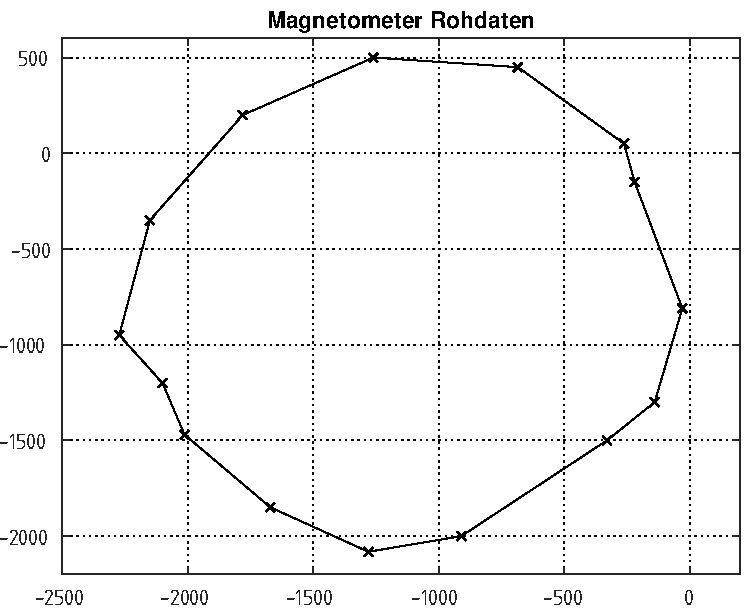
\includegraphics[width=\textwidth]{./img/qmc5883_raw.pdf}
                    \caption{Rohdaten}
                \end{subfigure}
                \begin{subfigure}[t]{.48\textwidth}
                    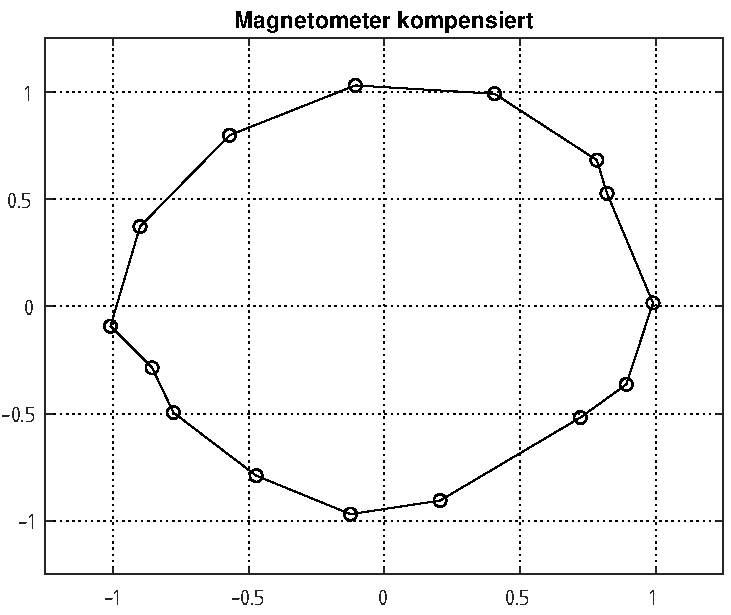
\includegraphics[width=\textwidth]{./img/qmc5883_compensated.pdf}
                    \caption{Kompensierte Werte}
                \end{subfigure}
                \caption{Kalibrierung des QMC5883L Magnetometers. Achsenbeschriftung ist zu beachten.}
                \label{fig:qmc_cal}
            \end{figure}
        
            Die Kompensation der Magnetfeldkomponenten erfolgt anschließend entsprechend der Formel:
            \begin{equation*}
                x_\star = (x - \bar{x}) \cdot \frac{2}{|\max{x} - \min{x}|}~~.
            \end{equation*}
            
            \paragraph{Berechnung der Kompassrichtung}\mbox{}\\
            Die Kompassrichtung kann aus zwei Magnetfeldkomponenten bestimmt werden. Für diese Anwendung wurden die X- und Y-Feldkomponenten gewählt. Nachdem die oben beschriebene Kalibrierung erfolgt ist, kann daraus über den $\arctan$ die Richtung des Feldvektors relativ zur Ausrichtung des Bauteils ermittelt werden:
            \begin{equation*}
                \theta = \arctan\left(\frac{y}{x}\right)
            \end{equation*}
            Zur Berücksichtigung des Falls $x < 0$ wird dabei die Funktion $\mathrm{atan2}$ eingesetzt:
            \begin{equation*}
                \theta = \mathrm{atan2}(x,\,y)
            \end{equation*}
            Da dies einen Winkel im Bereich $\theta \in [-\pi,\,\pi]$ liefert, muss eine Offsetkompensation und Umrechnung in Winkelgrade angewendet werden:
            \begin{equation*}
                \theta = 180\,^\circ + \mathrm{atan2}(x,\,y) \cdot \frac{180\,^\circ}{\pi}
            \end{equation*}
            Für die Darstellung als Festkommazahl mit $[\theta_\star] = 0.1\,^\circ$ kann der Faktor durch eine Integerkonstante ersetzt werden mit
            \begin{equation*}
                10 \cdot \frac{180\,^\circ}{\pi} \approx 573 \implies \theta_\star = (1800 + \mathrm{atan2}(x,\,y) \cdot 573) \cdot (0.1\,^\circ)
            \end{equation*}
        
            \paragraph{Temperatursensor}\mbox{}\\
            Der QMC5883 Sensor beinhaltet zusätzlich zum Magnetometer einen Temperatursensor zur internen Kompensation. Die Messwerte des Temperatursensors können zudem über die I\textsuperscript{2}C-Schnittstelle durch den Mikrocontroller ausgelesen werden.
            
            Der bereitgestellte Wert beschreibt dabei jedoch nur einen Offset zu einer intern kalibrierten Referenztemperatur. Diese ist im Datenblatt des Sensors nicht angegeben, und muss durch den Anwender empirisch ermittelt werden. In diesem Fall wurde ein Referenzwert von $34\,^\circ\mathrm{C}$ ermittelt.
            
            \paragraph{Sensordaten-Speicherstruktur}\mbox{}\\
            Die Kalibrierungsdaten zur Kompensation der X- und Y-Magnetfeldkomponenten, sowie der Temperatur-Referenzwert werden in einer Speicherstruktur im Arbeitsspeicher des Mikrocontrollers festgehalten (s. Listing~\ref{lst:qmc5883_typedef}). Die umgerechneten Messwerte werden für die Auswertung durch andere Programmteile bereitgestellt.
            
            \begin{lstlisting}[language=C,caption={Typdefinition für die Sensordatenstruktur des QMC5883L},label=lst:qmc5883_typedef]
/*!****************************************************************************
 * @brief
 * Sensordaten- und Konfigurationsstruktur für QMC5883
 *
 * @date  31.10.2019
 ******************************************************************************/
typedef struct tag_QMC5883_Sensor {
    /*! I2C Slaveadresse                                      */
    uint8_t ucSlaveAddr;
    
    /*! Kalibrierungsdaten                                    */
    struct {
        /*! Referenztemperatur in 0.1°C                       */
        int16_t iRefTemp;
        
        /*! Mittelwerte                                       */
        float fXComp;
        float fYComp;
        
        /*! Minima und Maxima der Felder während der Drehung  */
        int16_t iXMin;
        int16_t iXMax;
        int16_t iYMin;
        int16_t iYMax;
        
        /*! Normierungsfaktoren                               */
        float fXGain;
        float fYGain;
        
        /*! Anzahl der Messpunkte für die Kompensation        */
        uint16_t uiNumComp;
    } sCalib;
    
    /*! Kalibrierungsfahrt aktiv                              */
    bool bCalActive;
    
    /*! Rohdaten                                              */
    struct {
        /*! Feld in X-Richtung                                */
        int16_t iRawX;
        
        /*! Feld in Y-Richtung                                */
        int16_t iRawY;
        
        /*! Feld in Z-Richtung                                */
        int16_t iRawZ;
        
        /*! Temperatur-Rohwert                                */
        int16_t iRawTemp;
    } sRaw;
    
    /*! Umgerechnete Messdaten                                */
    struct {
        /*! Azimuth in 0.1°                                   */
        uint16_t uiAzimuth;
        
        /*! Temperatur in 0.01°C                              */
        int16_t iTemperature;
    } sMeasure;
} QMC5883_Sensor;
            \end{lstlisting}
        
        \subsubsection{MPU6050}\label{ssec:MPU6050}
            Das MPU6050 von InvenSense wird zur Bestimmung des Panel-Winkels eingesetzt. Im Baustein ist neben den MEMS-Accelerometern und -Gyroskopen für 3 Achsen zusätzlich ein Temperatursensor für die interne Kompensation implementiert. 
            
            Von den sieben Sensoren werden für diese Anwendung jedoch nur die drei Accelerometerachsen ausgewertet -- der Temperatursensor hatte sich in der Evaluierungsphase als zu ungenau erwiesen.
            
            In der Initialisierungsphase des Systems wird der Bausteim im ``Sleep''-Modus neu gestartet, und die ungenutzten Sensoren deaktiviert. Der Messbereich für das Accelerometer wird auf $\pm2\,\mathrm{g}$ parametriert.
            
            \paragraph{Aktivierung und Messdatenerfassung}\mbox{}\\
            In der Aufzeichnungsroutine des Mikrocontrollers, welche durch einen zeitgesteuerten Interrupt ausgelöst wird, wird der Sensor aus dem ``Sleep''-Modus geweckt und die Messdatenerfassung gestartet. Die Umsetzung der Messwerte ist erst nach einer kurzen Verzögerung von einigen Prozessorzyklen abgeschlossen, und wird durch ein ``Data Ready''-Flag in einem Sensor-Register signalisiert.
            
            Die rohen Messwerte vom Accelerometer werden anschließend in die Sensordaten-Struktur im Arbeitsspeicher des Mikrocontrollers eingelesen und in einen Winkel $\alpha_\star \in [-1800; 1800] \cdot (0.1\,^\circ)$ umgerechnet.
            
            \paragraph{Berechnung des Ausrichtungswinkels}\mbox{}\\
            Für die Ausrichtung des Panels werden die Y- und Z-Komponenten der Beschleunigung relativ zur Ausrichtung des Bausteins betrachtet. Für den  aus den Komponenten gebildeten Vektor wird über die $\arctan$-Funktion der Winkel zur Grundebene ermittelt:
            \begin{equation*}
                \alpha = \arctan\left(\frac{y}{z}\right)
            \end{equation*}
            Für die Behandlung des Falls $z < 0$ wird hier, ähnlich zur Berechnung der Kompassrichtung beim QMC5883, die $\mathrm{atan2}$-Funktion eingesetzt, welche einen Winkel $\alpha \in [-\pi, \pi]$ liefert.
            
            Dieser wird für die interne Darstellung in $[\alpha_\star] = 0.1\,^\circ$ umgerechnet.
            \begin{equation*}
                \alpha_\star = \mathrm{atan2}(z,\,y) \cdot \frac{1800\cdot (0.1\,^\circ)}{\pi}
            \end{equation*}
            Der konstante Faktor kann dabei durch eine Integerkonstante ersetzt werden:
            \begin{equation*}
                \alpha_\star = \mathrm{atan2}(z,\,y) \cdot 573 \cdot (0.1\,^\circ)~~.
            \end{equation*}
        
            \paragraph{Sensordaten-Speicherstruktur}\mbox{}\\
            Die Sensor-Messdaten werden in einem Strukturtyp im Arbeitsspeicher des Mikrocontrollers festgehalten (s. Listing~\ref{lst:mpu6050_typedef}) und durch unterschiedliche Programmteile ausgewertet. Über ein Feld für die Slaveadresse des Gerätes können bei Bedarf mehrere MPU6050-Sensoren angeschlossen werden\footnote{Hierzu muss der \texttt{AD0}-Pin des zweiten Bausteins an VCC angeschlossen werden~\cite[Kap 9.2]{ds_mpu6050}.}.
            
            \begin{lstlisting}[language=C,caption={Typdefinition für die Sensordatenstruktur des MPU6050},label=lst:mpu6050_typedef]
/*!****************************************************************************
 * @brief
 * Konfigurations- und Sensordatenstruktur für MPU6050
 *
 * @date  06.11.2019
 ******************************************************************************/
typedef struct tag_MPU6050_Sensor {
    /*! I2C Slaveadresse                                      */
    uint8_t ucSlaveAddr;
    
    /*! Temperaturmessungen aktiv                             */
    bool bMeasureTemp;
    
    /*! Rohdaten                                              */
    struct {
        /*! Rohwert für X-Beschleunigung                      */
        int16_t iRawX;
        
        /*! Rohwert für Y-Beschleunigung                      */
        int16_t iRawY;
        
        /*! Rohwert für Z-Beschleunigung                      */
        int16_t iRawZ;
        
        /*! Rohwert für Temperatur                            */
        int16_t iRawTemp;
    } sRaw;
    
    /*! Umgerechnete Messwerte                                */
    struct {
        /*! Einstellwinkel in 0.1°                            */
        struct {
            int iXZ;
            int iYZ;
        } sAngle;
    
        /*! Temperaturmesswert in 0.01°C                      */
        int16_t iTemperature;
    } sMeasure;
} MPU6050_Sensor;
            \end{lstlisting}
            
        \subsubsection{Anemometer und Windfahne}\label{ssec:Wind}
            Für dieses Projekt wurde ein neuer Aufbau für das Anemometer und die Windfahne eingesetzt, welcher als Schnittstelle zum Mikrocontroller eine analogen Spannung und ein digitales Gebersignal verwendet~\cite{ds_wind}. Somit konnte auf die Implementierung des proprietären Kommunikationsprotokolls für den Aufbau der Gruppe vom Vorjahr verzichtet werden.
            
            Auf der Seite des Mikrocontrollers werden zur Auswertung dementsprechend ein Kanal des ADU und ein Timer-Zähler Modul eingesetzt.
            
            \paragraph{Anemometer}
            Die Windgeschwindigkeit wird über das Drehgebersignal des Anemometers ermittelt. Hierzu wird in der Initialisierungsphase des Systems ein Hardware Timer des Mikrocontrollers als Impulszähler konfiguriert. Ein Impuls vom Anemometer auf dem Zähleingang inkrementiert den Zählerstand, welcher dann in einem festen Zeitintervall ausgewertet werden muss.
            
            Die Windgeschwindigkeit liegt dann in einer Einheit ``Impulse pro Zeitintervall'' vor -- praktischerweise wird der Zählerstand hier mit einer Periode von $1\,\mathrm{s}$ ausgewertet, wodurch die Windgeschwindigkeit entsprechend in einer Einheit ``Impulse pro Sekunde'' vorliegt.
            
            Aus den Datenblattangaben kann hierfür ein Umrechnungsfaktor ermittelt werden~\cite{ds_wind}: 
            \begin{equation*}
                v_w \approx n \cdot 2.4 \cdot \frac{\mathrm{km/h}}{\mathrm{s}}~~,
            \end{equation*}
            mit $n$ als Anzahl der Impulse im vergangenen Zeitintervall von $1\,\mathrm{s}$. Es gilt $[n] = 1\,\mathrm{pps}$.
        
            Für die interne Darstellung in $[v_{w\star}] = 1\,\mathrm{m/s}$ muss dieser Wert entsprechend umgerechnet werden mit
            \begin{equation*}
                1\,\mathrm{m/s} = 3.6\,\mathrm{km/h} = 2.4\,\frac{\mathrm{km/h}}{\mathrm{pps}}\ \cdot 3.6 \approx \frac{553}{2^6}\cdot\left(1\,\frac{\mathrm{m/s}}{\mathrm{pps}}\right)
            \end{equation*}
            in
            \begin{equation*}
                v_{w\star} = \left\lfloor\frac{n \cdot 553}{2^6}\right\rfloor \cdot (1\,\mathrm{m/s})~~.
            \end{equation*}
        
            Da die Erfassung der Windgeschwindigkeit ohnehin alle $1\,\mathrm{s}$ erfolgt, wird aus den Messwerten die mittlere Windgeschwindigkeit über die letzten 16 Sekunden, sowie die maximale Windgeschwindigkeit (z.B. Böen) in diesem Zeitfenster ermittelt.
            
            \paragraph{Windrichtung}\mbox{}\\
            Ein an der Windfahne angebrachter Magnet schließt je nach Windrichtung einen Widerstand oder zwei Widerstände in Parallelschaltung an einen Spannungsteiler. Über die Spannung am Ausgang des Teilers kann eine Zuordnung zu einer relativen Windrichtung erfolgen. Für die Messung wird in der Initialisierungsphase des Systems ein ADU-Kanal parametriert.
            
            Für die Zuordnung zwischen ADU-Wertebereich und Windrichtung wird eine \emph{Look-Up Table} eingesetzt. Die ADU-Werte hierfür wurden empirisch ermittelt. Die Windfahne ist mit acht Widerständen ausgestattet -- es können also 16 diskrete Werte als Windrichtung erkannt werden:
            \begin{figure}[H]
                \centering
                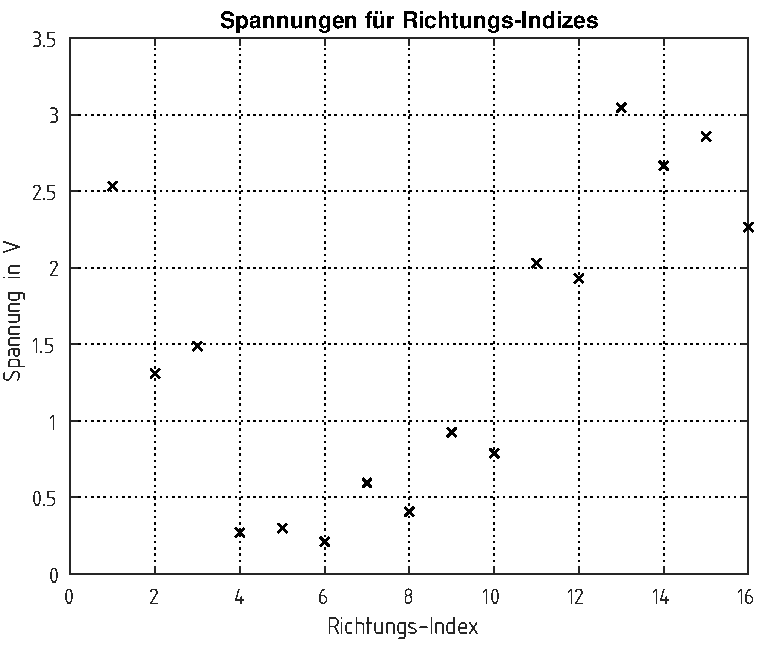
\includegraphics[width=.7\textwidth]{./img/Windfahne.pdf}
                \caption{ADU-Werte für 16 diskrete Richtungs-Werte (in positive Drehrichtung) der Windfahne}
                \label{fig:wv_adc}
            \end{figure}
        
            Die absolute Windrichtung kann nur dann ermittelt werden, wenn der digitale Kompass QMC5883 kalibriert wurde. Der über die LUT ermittelte Richtungsindex $k$ wird dann als Offset aufaddiert:
            \begin{equation*}
                \theta_w = \theta + k \cdot 22.5\,^\circ~~,
            \end{equation*}
            bzw. für die interne Darstellung mit $[\theta_{w\star}] = 0.1\,^\circ$:
            \begin{equation*}
                \theta_{w\star} = \theta_\star + k \cdot 225 \cdot (0.1\,^\circ)~~.
            \end{equation*}
        
            \paragraph{Sensordaten-Speicherstruktur}\mbox{}\\
            Die Messwerte für die Windgeschwindigkeit werden zur Mittelwertbildung in einem Ringspeicher mit 16 Elementen abgelegt. Zusätzlich die Böen-Windgeschwindigkeit in einer weiteren Speicherstelle abgelegt.
            
            \begin{lstlisting}[language=C,caption={Typdefinition für die Messdaten zur Bestimmung der Windrichtung und -geschwindigkeit},label=lst:wind_typedef]
/*!****************************************************************************
 * @brief
 *  Windsensor-Struktur
 *
 * @date  31.10.2019
 ******************************************************************************/
typedef struct tag_Wind_Sensor
{
    /*! Kalibrierungsdaten                                    */
    struct
    {
        /*! Timer-Abfrageintervall                            */
        uint16_t uiPollInterval;
    } sCalib;
    
    /*! Rohdaten                                              */
    struct
    {
        bool bRawDataUpdate;
        uint8_t ucHead;
        uint16_t auiRawVelocity[NUM_WIND_AVG];
        uint16_t uiRawDirection;
    } sRaw;
    
    /*! Umgerechnete Messwerte                                */
    struct
    {
        /*! Windgeschwindigkeit in m/s                        */
        uint16_t uiAvgVelocity;
        uint16_t uiMaxVelocity;
        
        /*! Windrichtung als Himmelsrichtung                  */
        Wind_Direction eDirection;
    } sMeasure;
} Wind_Sensor;
            \end{lstlisting}
            
        \subsubsection{Strom- und Spannungsmessung}
            Eine weitere Anforderung an die Wetterstation war die Aufzeichnung des Batterie-Ladezustandes in Form von Strom- und Spannungsmesswerten.
            
            Für die Spannungsmessung wird der ADU des Mikrocontrollers mit vorgeschalteten Spannungsteilern eingesetzt. Die Strommessung erfolgt mithilfe von ACS712-Stromsensoren, welche die Ströme in analoge Spannungswerte umsetzen, welche ebenfalls über den ADU eingelesen werden. Um den Mikrocontroller vor Überspannungen an den Analogeingängen zu schützen, sind Spannungsteiler mit Begrenzungsdioden vorgeschaltet.             
            
            Für die umgesetzten Spannungswerte wird eine Offsetkompensation (Strommessung) durchgeführt und die empirisch ermittelte Kennliniensteigung angewendet.
            
            \paragraph{Sensordaten-Speicherstruktur}\mbox{}\\
            Die Strom- und Spannungsmessung erfolgt für Akku und Solarpanel auf gleiche Weise, daher ist die Struktur so ausgelegt, dass sie universell für Kombinationen aus Strom- und Spannungssensoren eingesetzt werden kann. Zusätzlich werden in ihr die Nummern der jeweiligen ADU-Kanäle für die Umstellung des Analog-Mux festgehalten.
            
            \begin{lstlisting}[language=C,caption={Typdefinition für die Sensordatenstruktur der Strom- und Spannungssensoren},label=lst:power_typedef]
/*!****************************************************************************
 * @brief
 * Strukturdefinition für Strom- und Spannungsmessung
 *
 * @date 06.01.2020
 ******************************************************************************/
typedef struct tag_Power_Sensor {
    /*! Kalibrierungsdaten                                    */
    struct
    {
        /*! Nullpunktabgleich für die Strommessung als Rohw.  */
        uint16_t uiCurrZeroOffset;
        
        /*! Kennliniensteigung für den Strom in 1mA/lsb       */
        int16_t iCurrSlope;
        
        /*! Kennliniensteigung für die Spannung in 1mV/lsb    */
        uint16_t uiVoltSlope;
    } sCalib;
    
    /*! Konfiguration der ADC-Kanäle                          */
    struct
    {
        /*! Kanal für die Strommessung                        */
        ADC_Channel_TypeDef eCurr;
        
        /*! Kanal für die Spannungsmessung                    */
        ADC_Channel_TypeDef eVolt;
    } sChannel;
    
    /*! Rohdaten                                              */
    struct 
    {
        /*! ADC Rohwert für die Spannungsmessung              */
        uint16_t uiRawVolt;
        
        /*! ADC Rohwert für die Strommessung                  */
        uint16_t uiRawCurr;
    } sRaw;
    
    /*! Umgerechnete Messwerte                                */
    struct {
        /*! Spannungsmesswert in 1mV                          */
        uint16_t uiVolt;
        
        /*! Strommesswert in 1mA                              */
        int16_t iCurr;
    } sMeasure;
} Power_Sensor;
    \end{lstlisting}
            
    \subsection{GPS}\label{ssec:GPS}
        Das GPS-Modul sendet nach dem Einschalten der Versorgung sofort zyklisch Daten im NMEA 0183 Format über die UART-Schnittstelle an den Mikrocontroller. In der Initialisierungsphase wird hierfür ein GPIO-Pin für die Ansteuerung des Leistungs-MOSFETs der Versorgung, und die USART3 für den Datenempfang bei 9600 Baud (8N1) konfiguriert.
        
        Die eingehenden Daten werden mittels eines Interrupthandlers in einen Puffer eingelesen. Hierbei können einige Eigenschaften des NMEA 0183 Protokolls ausgenutzt werden, um die Konsistenz der Daten zu sichern:
        \begin{itemize}
            \item Jeder \emph{Sentence} beginnt mit dem Zeichen ``\texttt{\$}''.
            \item Der \emph{Sentence} endet mit dem Zeilenende, markiert durch ``\texttt{\textbackslash r\textbackslash n}''.
            \item Auf das Startzeichen folgt eine 5-stellige \emph{Sentence}-Kennung, gefolgt von einem Komma. Mögliche Werte hierfür sind bspw. ``\texttt{GPRMC}'' oder ``\texttt{GPGGA}''.
            \item Die Datenfelder des \emph{Sentence} sind durch Kommata getrennt.
        \end{itemize}
    
        \subsubsection{Interpretation der NMEA Sentences}
        Sobald die ersten 6 Zeichen eingelesen wurden, wird eine Abfrage gestartet, ob es sich hierbei um einen für die Auswertung relevanten \emph{Sentence} handelt. 
        
        Aus der Anforderungsspezifikation folgt, dass neben den Positionsdaten der aktuelle UTC-Zeitstempel und die Höhe über dem mittleren Meeresspiegel aus den GPS-Daten ermittelt werden sollen. Die relevanten NMEA Sentences hierfür sind:
        \begin{itemize}
            \item \texttt{GPRMC} -- ``Minimum recommended GPS/transit data''
            \item \texttt{GPGGA} -- ``Global Positioning System Fix Data''
        \end{itemize}
        Die zugehörigen Sentence-Formate werden nachfolgend kurz beschrieben. Bei der Auswertung werden die Sentences zeichenweise durchlaufen und eine Text-Interpretation durchgeführt.
        
        \paragraph{GPRMC: ``Minimum recommended GPS/transit data''}\mbox{}\\
        Beispiel:
        \begin{center}
            \$GPRMC,225446.00,A,5355.63,N,01002.26,W,082.5,054.7,031219,020.3,E*4D\textbackslash r\textbackslash n
        \end{center}
        Beschreibung:
        \begin{table}[H]
            \centering
            \begin{tabular}{|l|l|l|}
                \hline
                \textbf{Feld}   & \textbf{Beschreibung}                 & \textbf{Wert}\\
                \hline
                \$              & Startzeichen                          & \\
                GPRMC           & Sentence-Typ                          & \\
                225446.00       & UTC-Uhrzeit im Format hhmmss.zz       & 22:54:46 Z \\
                A               & Gültigkeit der Daten: \texttt{A} = gültig, \texttt{V} = kein Fix  & gültig\\
                5355.63,N       & Breitengrad im Format ddmm.mm, \texttt{N} = Nord, \texttt{S} = Süd & $\mathrm{N}\,53\,^\circ\,55.63\,'$\\
                01002.26,E      & Längengrad im Format dddmm.mm, \texttt{E} = Ost, \texttt{W} = West & $\mathrm{E}\,010\,^\circ\,02.26\,'$\\
                082.5           & Geschwindigkeit über Grund in Knoten &  $82.5\,\mathrm{kts}$    \\
                054.7           & Rechtweisender Kurs &  $054.7\,^\circ$   \\
                031219          & UTC-Datum im Format DDMMYY & 03.12.2019 \\
                020.3,E         & Variation, \texttt{E} = Ost, \texttt{W} = West  & $20.3\,^\circ$ Ost\\
                *4D             & Prüfsumme                            & \\
                \textbackslash r\textbackslash n & Zeilenende          & \\
                \hline
            \end{tabular}
            \caption{Beschreibung des \texttt{GPRMC} NMEA Sentence nach~\cite{nmea0183}}
            \label{nmea_gprmc} 
        \end{table}
                
        \paragraph{GPGGA: ``Global Positioning System Fix Data''}\mbox{}\\
        Beispiel:
        \begin{center}
            \$GPGGA,225446.00,5355.63,N,01002.26,E,1,09,1.5,419.3,M,39.5,M,,*66\textbackslash r\textbackslash n
        \end{center}
        
        Beschreibung:
        \begin{table}[H]
            \centering
            \begin{tabular}{|l|l|l|}
                \hline
                \textbf{Feld}   & \textbf{Beschreibung}                 & \textbf{Wert}\\
                \hline
                \$              & Startzeichen                          & \\
                GPGGA           & Sentence-Typ                          & \\
                225446.00       & UTC-Uhrzeit im Format hhmmss.zz       & 22:54:46 Z \\
                5355.63,N       & Breitengrad im Format ddmm.mm, \texttt{N} = Nord, \texttt{S} = Süd & $\mathrm{N}\,53\,^\circ\,55.63\,'$\\
                01002.26,E      & Längengrad im Format dddmm.mm, \texttt{E} = Ost, \texttt{W} = West & $\mathrm{E}\,010\,^\circ\,02.26\,'$\\
                1               & Fix Typ: 0 = kein Fix, 1 = GPS, 2 = differential GPS & GPS \\
                09              & Anzahl der empfangenen Satelliten     & 9\\
                1.5             & Relative genauigkeit der Position (HDOP) & \\
                419.3,M         & Höhe über dem mittleren Meeresspiegel (MSL) & $419.3\,\mathrm{m}$\\
                39.5,M          & Höhe über dem WGS84-Geoid & $39.5\,\mathrm{m}$ \\
                (leer)          & Zeit seit letztem DGPS-fix (bei GPS leer) & \\
                (leer)          & DGPS-Stationskennung (0000-4096, bei GPS leer) & \\
                *66             & Prüfsumme & \\
                \textbackslash r\textbackslash n & Zeilenende          & \\
                \hline
            \end{tabular}
            \caption{Beschreibung des \texttt{GPGGA} NMEA Sentence nach~\cite{nmea0183}}
            \label{nmea_gpgga} 
        \end{table}
    
        \subsubsection{Versorgung des GPS-Moduls}
            Um die Energieaufnahme des Systems zu verringern, wird das GPS-Modul nach dem ersten Positions-Fix abgeschaltet und nur in längeren Zeitabständen zur synchronisation der prozessorinternen Echtzeituhr reaktiviert.
            
            Die Abschaltung erfolgt über einen Leistungs-MOSFET auf der Versorgungsleitung des Moduls, welcher über einen GPIO-Pin des Controllers geschaltet wird.
    
        \subsubsection{GPS-Datenstruktur im Speicher}
        Die aus den oben beschriebenen Sentences eingelesenen Daten werden in einer Speicherstruktur für die Auswertung durch weitere Programmteile, beispielsweise die Sollwertberechnung für die Nachführung des Solarpanels, bereitgestellt.
        
    \subsection{Bluetooth}\label{ssec:AT_Commands}
        Für die drahtlose Kommunikation mit einem Rechner wird ein Serial-over-Bluetooth Umsetzermodul eingesetzt. Es ist am Mikrocontroller an der USART2-Schnittstelle angeschlossen und kann, ähnlich wie das GPS-Modul, über einen Leistungs-MOSFET an der Versorgung abgeschaltet werden.
        
        Nach Installation des Gerätetreibers am PC erscheint die Schnittstelle als virtueller COM-Port. Die Kommunikation kann dann über ein Terminal-Programm wie \emph{PuTTY} oder die im Kapitel~\ref{sec:benutzeroberflaeche} beschriebene grafische Benutzeroberfläche erfolgen.
        
        \subsubsection{AT-Befehlssatz}
        Für die Kommunikation wurde ein auf dem \emph{Hayes command protocol} basierender AT-Befehlssatz implementiert. Merkmal des Protokolls ist, dass Befehle vom Benutzerterminal stets mit der Zeichenfolge ``\texttt{AT}'' beginnen, und mit der Zeichenfolge ``\texttt{\textbackslash r}'' enden.
        
        Nachfolgend werden einige der verfügbaren Befehle beschrieben.
        
        \paragraph{AT: Verbindungsstatus prüfen}\mbox{}\\
        Der Befehl ``\texttt{AT}'' kann zur Überprüfung des Verbindungsstatus genutzt werden. Die Wetterstation beantwortet alle Statusanfragen mit ``\texttt{OK}''.
        
        \begin{table}[H]
            \centering
            \begin{tabular}{|p{0.25\textwidth}|p{0.5\textwidth}|}
                \hline
                \textbf{Execute-Command} &\textbf{Antwort} \\
                \hline
                \texttt{AT} & \texttt{OK}\\
                \hline
            \end{tabular}
        \end{table}
    
        \paragraph{ATE: Remote-Echo aktivieren oder deaktivieren}\mbox{}\\
        Wenn die Befehlseingabe manuell über ein Terminalprogramm erfolgt (bspw. \emph{PuTTY}), ist eine Ausgabe der getippten Zeichen für den Anwender hilfreich. Diese \emph{Remote Echo}-Funktion kann über den ``\texttt{ATE}''-Befehl aktiviert werden.
        
        \begin{table}[H]
            \centering
            \begin{tabular}{|p{0.25\textwidth}|p{0.5\textwidth}|}
                \hline
                \textbf{Write-Command} &\textbf{Antwort} \\
                \hline
                \texttt{ATE<n>} & \texttt{OK}\\
                \hline
            \end{tabular}\\[3mm]
            \begin{tabular}{|p{0.25\textwidth}|p{0.5\textwidth}|}
                \hline
                \textbf{Feld}       & \textbf{Beschreibung}\\
                \hline
                \texttt{<n>}      & Aktivierungszustand der Remote-Echo Funktion. 0: ausgeschaltet, 1: eingeschaltet \\
                \hline
            \end{tabular}
        \end{table}
    
        \paragraph{AT+CTEMP: Temperaturmesswerte}\mbox{}\\
        Die aktuellen Temperaturmesswerte können mithilfe des ``\texttt{AT+CTEMP}''-Befehls ausgelesen werden.
        
        \begin{table}[H]
            \centering
            \begin{tabular}{|p{0.25\textwidth}|p{0.5\textwidth}|}
                \hline
                \textbf{Read-Command} &\textbf{Antwort} \\
                \hline
                \texttt{AT+CTEMP?}  & \texttt{+CTEMP: <bme>,<cpu>,<qmc>,<mpu>}\\
                                    & \texttt{OK}\\
                \hline
            \end{tabular}\\[3mm]
            \begin{tabular}{|p{0.25\textwidth}|p{0.5\textwidth}|}
                \hline
                \textbf{Feld}       & \textbf{Beschreibung}\\
                \hline
                \texttt{<bme>}      & Temperatur vom BME280 in $0.01\,^\circ\mathrm{C}$\\
                \texttt{<cpu>}      & CPU-Temperatur in $0.01\,^\circ\mathrm{C}$\\
                \texttt{<qmc>}      & Temperatur vom QMC5883L in $0.01\,^\circ\mathrm{C}$\\
                \texttt{<mpu>}      & Temperatur vom MPU6050 in $0.01\,^\circ\mathrm{C}$\\
                \hline
            \end{tabular}
        \end{table}
    
        \paragraph{AT+CPRES: Luftdruck}\mbox{}\\
        Über den ``\texttt{AT+CPRES}''-Befehl kann der Luftdruck-Messwert vom BME280 ausgelesen werden.
        
        \begin{table}[H]
            \centering
            \begin{tabular}{|p{0.25\textwidth}|p{0.5\textwidth}|}
                \hline
                \textbf{Read-Command} &\textbf{Antwort} \\
                \hline
                \texttt{AT+CPRES?}  & \texttt{+CPRES: <bme>}\\
                & \texttt{OK}\\
                \hline
            \end{tabular}\\[3mm]
            \begin{tabular}{|p{0.25\textwidth}|p{0.5\textwidth}|}
                \hline
                \textbf{Feld}       & \textbf{Beschreibung}\\
                \hline
                \texttt{<bme>}      & Luftdruck-Messwert vom BME280 in $1\,\mathrm{Pa}$\\
                \hline
            \end{tabular}
        \end{table}
    
        \paragraph{AT+CHUM: Relative Luftfeuchtigkeit}\mbox{}\\
        Die durch den BME280 gemessene, relative Luftfeuchtigkeit kann über den ``\texttt{AT+CHUM}''-Befehl ausgelesen werden.
        
        \begin{table}[H]
            \centering
            \begin{tabular}{|p{0.25\textwidth}|p{0.5\textwidth}|}
                \hline
                \textbf{Read-Command} &\textbf{Antwort} \\
                \hline
                \texttt{AT+CHUM?}  & \texttt{+CHUM: <bme>}\\
                & \texttt{OK}\\
                \hline
            \end{tabular}\\[3mm]
            \begin{tabular}{|p{0.25\textwidth}|p{0.5\textwidth}|}
                \hline
                \textbf{Feld}       & \textbf{Beschreibung}\\
                \hline
                \texttt{<bme>}      & Relative Luftfeuchtigkeit in $0.01\,\%$\\
                \hline
            \end{tabular}
        \end{table}
    
        \paragraph{AT+CWIND: Windrichtung und -geschwindigkeit}\mbox{}\\
        Die Windgeschwindigkeit und die Windrichtung werden über den Befehl ``\texttt{AT+CWIND}'' abgefragt.
        
        \begin{table}[H]
            \centering
            \begin{tabular}{|p{0.25\textwidth}|p{0.5\textwidth}|}
                \hline
                \textbf{Read-Command} &\textbf{Antwort} \\
                \hline
                \texttt{AT+CWIND?}  & \texttt{+CWIND: <dir>,<spd>}\\
                & \texttt{OK}\\
                \hline
            \end{tabular}\\[3mm]
            \begin{tabular}{|p{0.25\textwidth}|p{0.5\textwidth}|}
                \hline
                \textbf{Feld}       & \textbf{Beschreibung}\\
                \hline
                \texttt{<dir>}      & Windrichtung in $0.1\,^\circ$\\
                \texttt{<spd>}      & Windgeschwindigkeit in $1\,\mathrm{m/s}$\\
                \hline
            \end{tabular}
        \end{table}
    
        \paragraph{AT+CTIME: Echtzeituhr}\mbox{}\\
        Über den ``\texttt{AT+CTIME}''-Befehl können Datum und Uhrzeit der internen Echtzeituhr ausgelesen und überschrieben werden.
        
        \begin{table}[H]
            \centering
            \begin{tabular}{|p{0.25\textwidth}|p{0.5\textwidth}|}
                \hline
                \textbf{Read-Command} &\textbf{Antwort} \\
                \hline
                \texttt{AT+CTEMP?}  & \texttt{+CTIME: <YY>,<MM>,<DD>,<hh>,<mm>, <ss>}\\
                & \texttt{OK}\\
                \hline
            \end{tabular}\\[3mm]
            \begin{tabular}{|p{0.25\textwidth}|p{0.5\textwidth}|}
                \hline
                \textbf{Write-Command} &\textbf{Antwort} \\
                \hline
                \texttt{AT+CTIME=<YY>, <MM>,<DD>,<hh>, <mm>,<ss>} & \texttt{OK}\\
                \hline
            \end{tabular}\\[3mm]
            \begin{tabular}{|p{0.25\textwidth}|p{0.5\textwidth}|}
                \hline
                \textbf{Feld}       & \textbf{Beschreibung}\\
                \hline
                \texttt{<YY>}       & Jahr 0 bis 99 \\
                \texttt{<MM>}       & Monat 1 bis 12 \\
                \texttt{<DD>}       & Tag 1 bis 31 \\
                \texttt{<hh>}       & Stunde 0 bis 23 (UTC) \\
                \texttt{<mm>}       & Minute 0 bis 59 \\
                \texttt{<ss>}       & Sekunde 0 bis 59 \\
                \hline
            \end{tabular}
        \end{table}
    
        \paragraph{AT+CALIGN: Ausrichtung des Panels}
        Die aktuelle Ausrichtung des Solarpanels, wie sie über den Kompass und den Neigungssensor ermittelt wurde, kann über den ``\texttt{AT+CALIGN}''-Befehl ausgelesen werden.
        
        \begin{table}[H]
            \centering
            \begin{tabular}{|p{0.25\textwidth}|p{0.5\textwidth}|}
                \hline
                \textbf{Read-Command} &\textbf{Antwort} \\
                \hline
                \texttt{AT+CALIGN?}  & \texttt{+CALIGN: <azm>,<zen>}\\
                & \texttt{OK}\\
                \hline
            \end{tabular}\\[3mm]
            \begin{tabular}{|p{0.25\textwidth}|p{0.5\textwidth}|}
                \hline
                \textbf{Feld}       & \textbf{Beschreibung}\\
                \hline
                \texttt{<azm>}      & Azimuth in $0.1\,^\circ$\\
                \texttt{<zen>}      & Zenit in $0.1\,^\circ$\\
                \hline
            \end{tabular}
        \end{table}
    
        \paragraph{AT+CGNSPOS: GPS-Position}\mbox{}\\
        Nachdem ein gültiges Fix vom GPS-Modul erhalten wurde, kann die Position über den ``\texttt{AT+CGNSPOS}''-Befehl ausgelesen werden. Sollte kein Fix gefunden werden können (bspw. innerhalb von Gebäuden), kann über diesen Befehl eine Position manuell vorgegeben werden.
        
        \begin{table}[H]
            \centering
            \begin{tabular}{|p{0.25\textwidth}|p{0.5\textwidth}|}
                \hline
                \textbf{Read-Command} &\textbf{Antwort} \\
                \hline
                \texttt{AT+CGNSPOS?}  & \texttt{+CGNSPOS: <lat>,<lon>,<alt>}\\
                & \texttt{OK}\\
                \hline
            \end{tabular}\\[3mm]
            \begin{tabular}{|p{0.25\textwidth}|p{0.5\textwidth}|}
                \hline
                \textbf{Write-Command} &\textbf{Antwort} \\
                \hline
                \texttt{AT+CGNSPOS=<lat>, <lon>[,<alt>]} & \texttt{OK}\\
                \hline
            \end{tabular}\\[3mm]
            \begin{tabular}{|p{0.25\textwidth}|p{0.5\textwidth}|}
                \hline
                \textbf{Feld}       & \textbf{Beschreibung}\\
                \hline
                \texttt{<lat>}      & Breitengrad $0.0001\,^\circ\,\mathrm{N}$\\
                                    & ($\mathrm{S}$ durch negatives Vorzeichen)\\
                \texttt{<lon>}      & Längengrad in $0.0001\,^\circ\,\mathrm{E}$\\
                                    & ($\mathrm{W}$ durch negatives Vorzeichen)\\
                \texttt{<alt>}      & (optional) Höhe über MSL in $0.1\,\mathrm{m}$\\
                \hline
            \end{tabular}
        \end{table}
        
        \paragraph{AT+CPWR: Strom- und Spannungsmesswerte}
        Die gemessenen Ströme und Spannungen an dem Akku und der Solarzelle können über den ``\texttt{AT+CPWR}''-Befehl ausgelesen werden.
        
        \begin{table}[H]
            \centering
            \begin{tabular}{|p{0.25\textwidth}|p{0.5\textwidth}|}
                \hline
                \textbf{Read-Command} &\textbf{Antwort} \\
                \hline
                \texttt{AT+CPWR?}  & \texttt{+CPWR: <v\_bat>,<i\_bat>,<v\_solar>, <i\_solar>,<v\_sys>}\\
                & \texttt{OK}\\
                \hline
            \end{tabular}\\[3mm]
            \begin{tabular}{|p{0.25\textwidth}|p{0.5\textwidth}|}
                \hline
                \textbf{Feld}       & \textbf{Beschreibung}\\
                \hline
                \texttt{<v\_bat>}   & Akkuspannung in $1\,\mathrm{mV}$\\
                \texttt{<i\_bat>}   & Ladestrom in $1\,\mathrm{mA}$\\
                \texttt{<v\_solar>} & Panelspannung in $1\,\mathrm{mV}$\\
                \texttt{<i\_solar>} & Panelstrom in $1\,\mathrm{mA}$\\
                \texttt{<v\_sys>}   & Systemspannung in $1\,\mathrm{mV}$, konstant $3.3\,\mathrm{V}$\\
                \hline
            \end{tabular}
        \end{table}
        
        \paragraph{AT+CINTV: Messintervall}\mbox{}\\
        Die Periodendauer, mit welcher die Sensoren periodisch ausgewertet werden, kann über den ``\texttt{AT+CINTV}''-Befehl angepasst werden.
        
        \begin{table}[H]
            \centering
            \begin{tabular}{|p{0.25\textwidth}|p{0.5\textwidth}|}
                \hline
                \textbf{Write-Command} &\textbf{Antwort} \\
                \hline
                \texttt{AT+CINTV=<int>} & \texttt{OK}\\
                \hline
            \end{tabular}\\[3mm]
            \begin{tabular}{|p{0.25\textwidth}|p{0.5\textwidth}|}
                \hline
                \textbf{Feld}    & \textbf{Beschreibung}\\
                \hline
                \texttt{<int>}   & Messintervall in $1\,\mathrm{s}$\\
                \hline
            \end{tabular}
        \end{table}
    
        \paragraph{AT+CGUI: Daten für die grafische Benutzeroberfläche}\mbox{}\\
        Die grafische Benutzeroberfläche ruft die letzten gespeicherten Messwerte über den ``\texttt{AT+CGUI}''-Befehl ab.
        \begin{table}[H]
            \centering
            \begin{tabular}{|p{0.25\textwidth}|p{0.5\textwidth}|}
                \hline
                \textbf{Read-Command} &\textbf{Antwort} \\
                \hline
                \texttt{AT+CGUI?}  & \texttt{+CGUI: <YY>,<MM>,<DD>,<hh>,<mm>, <ss>,<t\_bme>,<t\_cpu>,<t\_qmc>, <t\_mpu>,<w\_dir>,<w\_spd>,<pres>, <hum>,<zen>,<azm>,<lat>,<lon>, <alt>,<v\_bat>,<i\_bat>,<v\_solar>, <i\_solar>,<v\_sys>}\\
                & \texttt{+CGUI: ...}\\
                & \texttt{OK}\\
                \hline
            \end{tabular}\\[3mm]
            \begin{tabular}{|p{0.25\textwidth}|p{0.5\textwidth}|}
                \hline
                \textbf{Feld}       & \textbf{Beschreibung}\\
                \hline
                \texttt{<YY>}       & Jahr 0 bis 99 \\
                \texttt{<MM>}       & Monat 1 bis 12 \\
                \texttt{<DD>}       & Tag 1 bis 31 \\
                \texttt{<hh>}       & Stunde 0 bis 23 (UTC) \\
                \texttt{<mm>}       & Minute 0 bis 59 \\
                \texttt{<ss>}       & Sekunde 0 bis 59 \\
                \texttt{<t\_bme>}   & Temperatur vom BME280 in $0.01\,^\circ\mathrm{C}$\\
                \texttt{<t\_cpu>}   & CPU-Temperatur in $0.01\,^\circ\mathrm{C}$\\
                \texttt{<t\_qmc>}   & Temperatur vom QMC5883L in $0.01\,^\circ\mathrm{C}$\\
                \texttt{<t\_mpu>}   & Temperatur vom MPU6050 in $0.01\,^\circ\mathrm{C}$\\
                \texttt{<w\_dir>}   & Windrichtung in $0.1\,^\circ$\\
                \texttt{<w\_spd>}   & Windgeschwindigkeit in $1\,\mathrm{m/s}$\\
                \texttt{<pres>}      & Luftdruck-Messwert vom BME280 in $1\,\mathrm{Pa}$\\
                \texttt{<hum>}      & Relative Luftfeuchtigkeit in $0.01\,\%$\\
                \texttt{<zen>}      & Zenit in $0.1\,^\circ$\\
                \texttt{<azm>}      & Azimuth in $0.1\,^\circ$\\
                \texttt{<lat>}      & Breitengrad $0.0001\,^\circ\,\mathrm{N}$\\
                & ($\mathrm{S}$ durch negatives Vorzeichen)\\
                \texttt{<lon>}      & Längengrad in $0.0001\,^\circ\,\mathrm{E}$\\
                & ($\mathrm{W}$ durch negatives Vorzeichen)\\
                \texttt{<alt>}      & (optional) Höhe über MSL in $0.1\,\mathrm{m}$\\
                \texttt{<v\_bat>}   & Akkuspannung in $1\,\mathrm{mV}$\\
                \texttt{<i\_bat>}   & Ladestrom in $1\,\mathrm{mA}$\\
                \texttt{<v\_solar>} & Panelspannung in $1\,\mathrm{mV}$\\
                \texttt{<i\_solar>} & Panelstrom in $1\,\mathrm{mA}$\\
                \texttt{<v\_sys>}   & Systemspannung in $1\,\mathrm{mV}$, konstant $3.3\,\mathrm{V}$\\
                \hline
            \end{tabular}
            \label{tab:at_cgui}
        \end{table}
    
        \paragraph{AT+CWKUP: Wakeup-Task manuell Ausführen}\mbox{}\\
        Der Wakeup-Task kann durch Aufruf des ``\texttt{AT+CWKUP}''-Befehls manuell ausgelöst werden.
        
        \begin{table}[H]
            \centering
            \begin{tabular}{|p{0.25\textwidth}|p{0.5\textwidth}|}
                \hline
                \textbf{Execute-Command} &\textbf{Antwort} \\
                \hline
                \texttt{AT+CWKUP}  & \texttt{OK}\\
                \hline
            \end{tabular}
        \end{table}
    
        \paragraph{AT+CTRACK: Nachführung des Panels}\mbox{}\\
        Die Nachführung des Solarpanels kann über den ``\texttt{AT+CTRACK}''-Befehl aktiviert werden. Sie ist beim Systemstart aus Sicherheitsgründen deaktiviert.
        
        \begin{table}[H]
            \centering
            \begin{tabular}{|p{0.25\textwidth}|p{0.5\textwidth}|}
                \hline
                \textbf{Read-Command} &\textbf{Antwort} \\
                \hline
                \texttt{AT+CTRACK?}  & \texttt{+CTRACK: <stat>}\\
                & \texttt{OK}\\
                \hline
            \end{tabular}\\[3mm]
            \begin{tabular}{|p{0.25\textwidth}|p{0.5\textwidth}|}
                \hline
                \textbf{Write-Command} &\textbf{Antwort} \\
                \hline
                \texttt{AT+CTRACK=<stat>} & \texttt{OK}\\
                \hline
            \end{tabular}\\[3mm]
            \begin{tabular}{|p{0.25\textwidth}|p{0.5\textwidth}|}
                \hline
                \textbf{Feld}       & \textbf{Beschreibung}\\
                \hline
                \texttt{<stat>}    & Aktivierungszustand der Nachführung. 0: ausgeschaltet, 1: eingeschaltet\\
                \hline
            \end{tabular}
        \end{table}
    
        \paragraph{AT+CTURN: Manuelle Turm-Ausrichtung}\mbox{}\\
        Der Turm kann manuell mithilfe des ``\texttt{AT+CTURN}''-Befehls zeitgesteuert in eine vorgegebene Richtung gedreht werden. Außerdem wird über diesen Befehl die Kalibrierung des Magnetomers QMC5883L gestartet.
        
        \begin{table}[H]
            \centering
            \begin{tabular}{|p{0.25\textwidth}|p{0.5\textwidth}|}
                \hline
                \textbf{Write-Command} &\textbf{Antwort} \\
                \hline
                \texttt{AT+CTURN=<dir>} & \texttt{OK}\\
                \hline
            \end{tabular}\\[3mm]
            \begin{tabular}{|p{0.25\textwidth}|p{0.5\textwidth}|}
                \hline
                \textbf{Feld}       & \textbf{Beschreibung}\\
                \hline
                \texttt{<dir>}      & Richtung des Turms relativ zur Startposition in $0.1\,^\circ$.\\
                                    & \texttt{'C'} zum Start der Kalibrierung\\
                \hline
            \end{tabular}
        \end{table}
    
        \subsubsection{Energiesparmaßnahmen}
        Das Bluetooth-Modul hat im Sendebetrieb einen hohen Energieverbrauch (etwa $500\,\mathrm{mW}$). Es wird daher nach einer längeren Zeit ohne aktive Verbindung über einen Leistungs-MOSFET abgeschaltet.
        
        Damit dennoch ohne physikalischen Zugriff eine Verbindung mit der Wetterstation aufgebaut werden kann, wird das Bluetooth-Modul in regelmäßigen Zeitabständen für etwa $30\,\mathrm{s}$ im ``Advertise''-Modus eingeschaltet. In dieser Zeit ist das Modul für andere Bluetooth-Endgeräte in der Umgebung als ``\texttt{Wetterstation\_1a}'' sichtbar.
        
        Alternativ kann das Bluetooth-Modul durch Drücken des blauen Tasters an der Hauptplatine für länger als $1\,\mathrm{s}$ manuell aktiviert werden.
           
        \subsubsection{Pairing-Daten}
        Bei der erstmaligen Verbindung eines PCs mit der Wetterstation muss zunächst ein \emph{Pairing} zwischen dem Bluetooth-Modul und dem Rechner erfolgen. Hierbei muss am PC ein vierstelliger Pin-Code eingegeben werden, um die Verbindung zu aktivieren: \textbf{\texttt{1234}}
    
    \subsection{Messdatenprotokoll auf einer SD-Karte}\label{ssec:SD_Card}
        Die Messdaten werden bei jeder Aufzeichnung zusätzlich auf der SD-Karte in der Textdatei ``\texttt{LOG.TXT}'' im CSV-Format abgespeichert. Jede Zeile ist dabei nach folgendem Schema zusammengestellt:
        \begin{center}
            \texttt{<YYYY>-<MM>-<DD>T<hh>:<mm>:<ss>Z,<t\_bme>,<t\_cpu>,<t\_qmc>, <t\_mpu>,<pres>,<hum>,<w\_dir>,<w\_spd>,<azm>,<zen>,<lat>, <lon>,<alt>,<v\_bat>,<i\_bat>,<v\_solar>,<i\_solar>}
        \end{center}
    
        Die Formatierung der einzelnen Felder ist identisch zur Ausgabe des AT-Befehls ``\texttt{AT+CGUI}'', welche zuvor auf Seite~\pageref{tab:at_cgui} dokumentiert wurde.
        
    \subsection{Motorsteuerung}
        Die Motorsteuerung nutzt einen schnellen Timer-Interrupt mit einer Periode von $100\,\mathrm{ms}$ zur Regelung der Panelausrichtung. Die Fahrt erfolgt dabei zeitgesteuert, und wird nach Erreichen der Sollposition mithilfe des Magnetometers QMC5883L für Abweichungen kompensiert.
        
        Bei gleichzeitigen Sollwertänderungen für Panel- und Turmausrichtung wird zuerst das Panel verfahren. Der Turm wird erst nach Erreichen der Sollposition für die Panel-Achse verfahren, um übermäßig hohe Stromspitzen zu vermeiden.
        
        \subsubsection{Referenzfahrt für die Panelausrichtung}
        Nach der Initialisierung führt die Motorsteuerung eine Referenzfahrt auf der Panel-Achse aus, um einen Referenzwert für die Ausrichtung des Solarpanels entlang der Querachse zu erhalten. Das Panel wird dazu so lange nach unten gefahren, bis der Endlagenschalter auslöst.
        
        \subsubsection{Sicherheitsfunktion}
        Die Sicherheitsfunktion kann über den ``\texttt{ST}''-Schaltereingang ausgelöst werden. Hierdurch werden alle Treibersignale ausgeschaltet und die Motorsteuerung gegen Wiedereinschalten gesperrt. Dieser Zustand kann nur durch einen Neustart des Systems zurückgesetzt werden.
               
    \subsection{Statusanzeige über LEDs}
        Die Wetterstation verfügt über drei verschiedenfarbige Leuchtdioden, welche am Gehäuse der Hauptplatine montiert sind. Hierüber werden einige wichtige Systemzustände angezeigt. Die Bedeutung der Blink-Pattern wird nachfolgend kurz beschrieben. Die Pattern werden alle $1.5\,\mathrm{s}$ wiederholt.
        
        \subsubsection{Grüne LED: Systemstatus}
        Die grüne LED zeigt den Systemzustand der Wetterstation an. 
        \begin{table}[H]
            \centering
            \begin{tabular}{|l|l|}
                \hline
                \textbf{Blink-Pattern}  & \textbf{Zustand}  \\
                \hline
                1x kurzes Blinken       & Energiesparmodus aktiv \\
                2x kurzes, 1x langes Blinken & Wakeup-Task wurde ausgeführt\\
                Blinken ohne Pause      & Fehler beim Systemstart\\
                \hline
            \end{tabular}
        \end{table}
        
        \subsubsection{Blaue LED: Bluetooth}
        Der Aktivierungszustand des Bluetooth-Moduls wird über die blaue LED signalisiert.
        \begin{table}[H]
            \centering
            \begin{tabular}{|l|l|}
                \hline
                \textbf{Blink-Pattern}  & \textbf{Zustand}  \\
                \hline
                ausgeschaltet           & Modul ausgeschaltet. \\
                2x kurzes Blinken       & ``Advertise''-Modus. Nicht verbunden.\\
                dauerhaft ein           & Verbindung aktiv. \\
                \hline
            \end{tabular}
        \end{table}
        
        \subsubsection{Gelbe LED: Motorsteuerung}
        Die gelbe LED zeigt den aktuellen Zustand der Motorsteuerung an.
        \begin{table}[H]
            \centering
            \begin{tabular}{|l|l|}
                \hline
                \textbf{Blink-Pattern}  & \textbf{Zustand}  \\
                \hline
                ausgeschaltet           & Motorsteuerung deaktiviert. \\
                1x kurzes, 1x langes Blinken & Referenzfahrt angefordert.\\
                2x kurzes Blinken       & Referenzfahrt beendet.\\
                1x kurzes Blinken       & Motorsteuerung aktiv.\\
                Blinken ohne Pause      & Sicherheitsfunktion ausgelöst.\\
                \hline
            \end{tabular}
        \end{table}